\section{Learning Framework}
At previous KDD Cups, winning solutions either combined only single models without further combining ensemble models \cite{guyon2009analysis, yu2010feature} or combined ensemble models based on public leaderboard scores, which are not available in practice \cite{chen2011, wu2012two}.

However, we were able to combine ensemble models in multiple stages without overfitting to training data or using public leaderboard scores by using our learning framework.  Our learning framework consists of the stratified cross validation (CV) and multi-stage ensemble.

\subsection{Model Validation}

\begin{figure}
  \centering
    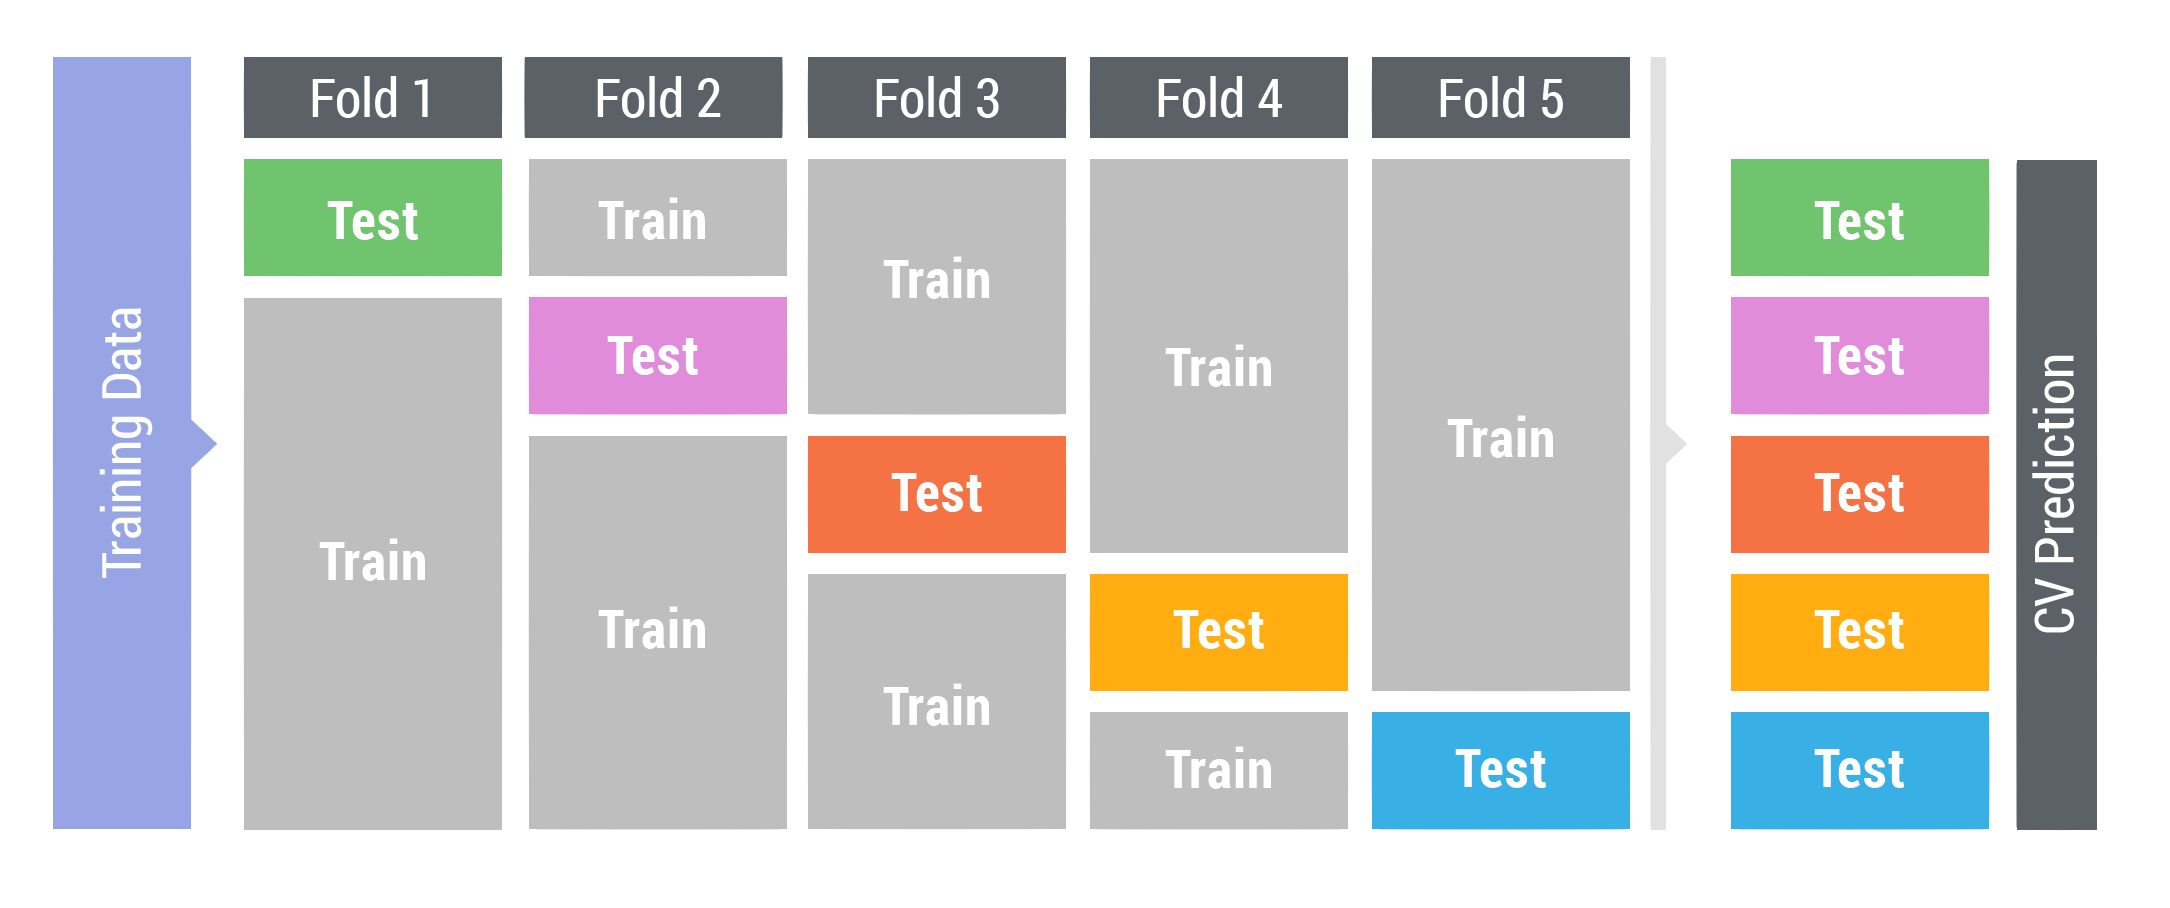
\includegraphics[width=0.5 \textwidth]{cv}
    \caption{5-fold CV.}
\end{figure}

We used stratified 5-fold CV for model validation and ensemble.
As shown in Figure 3, training data were split into 5 folds while the sample size and dropout rate were preserved across the folds.

For validation, each of single and ensemble models was trained 5 times. Each time, 1 fold was held out and the remaining 5 folds were used for training. Then, predictions for the hold-out folds were combined and formed the model's CV prediction. CV predictions were used as inputs for ensemble model training as well as the model's CV score calculation.

For test, each of single and ensemble models was retrained with whole training data. Then predictions for test data were used as inputs for ensemble prediction as well as for submission. 

\subsection{Multi-Stage Ensemble}

\begin{figure}[!h]
  \centering
    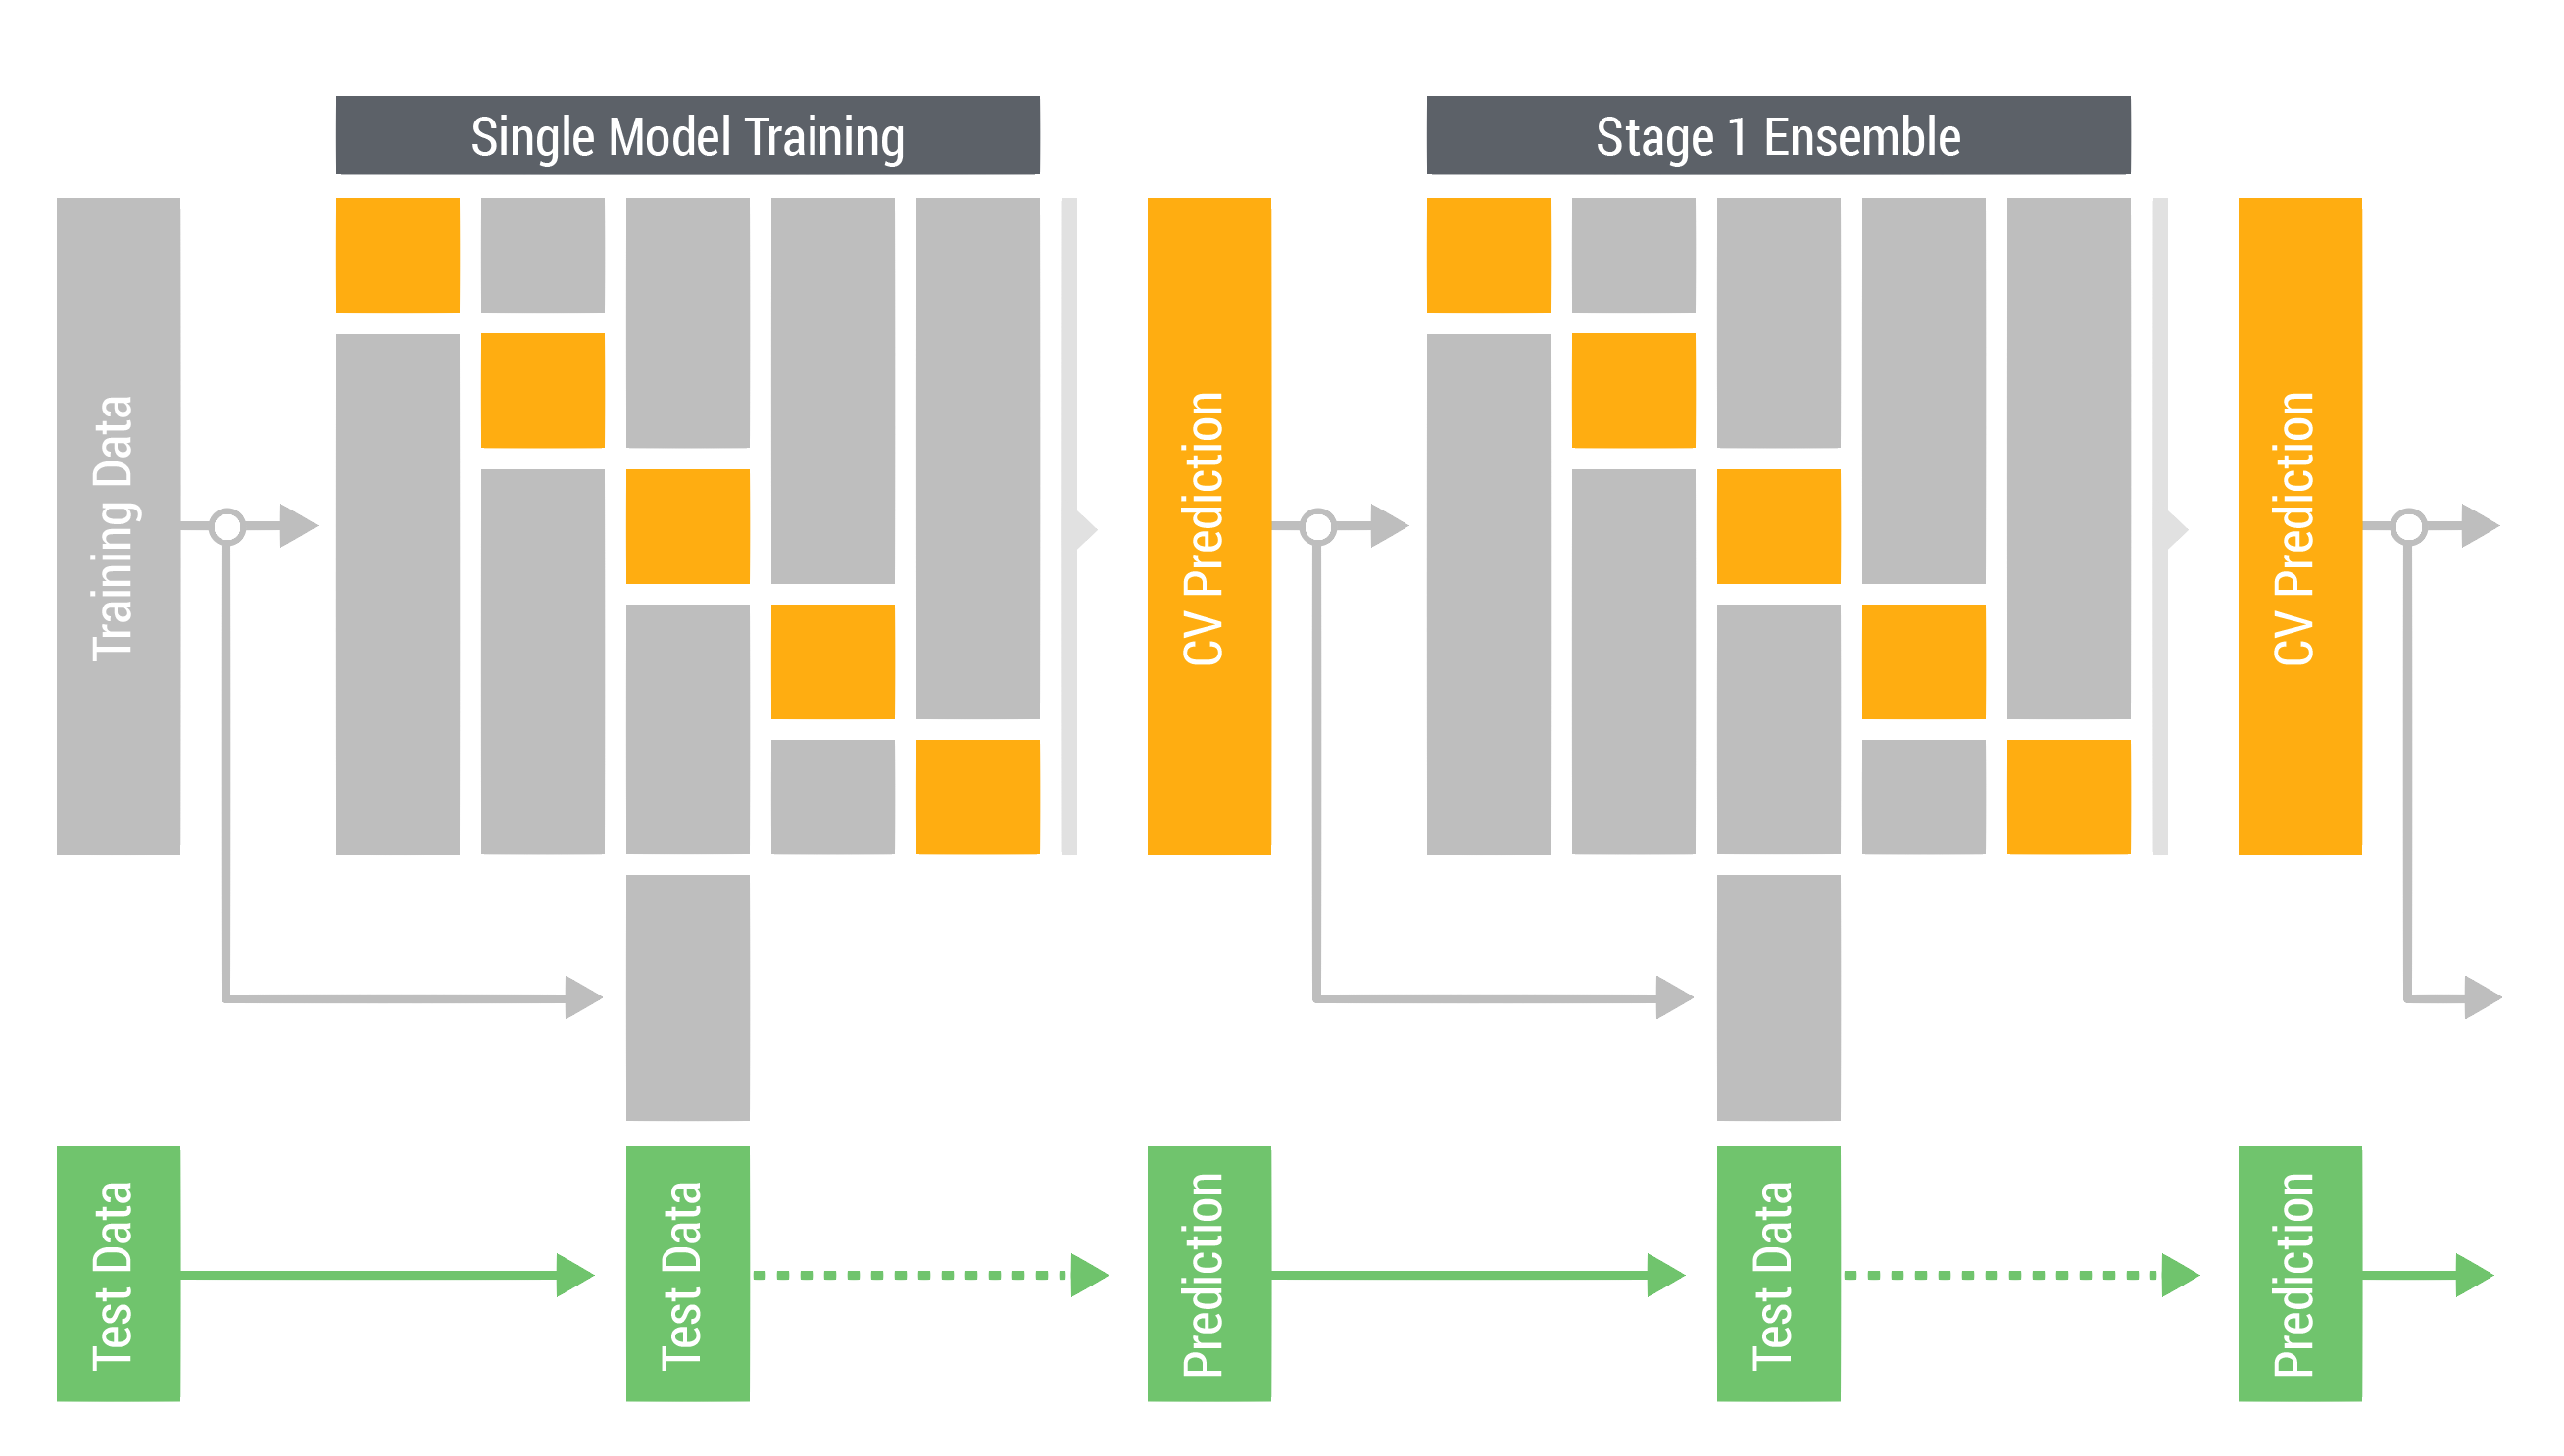
\includegraphics[width=0.5 \textwidth]{cv_ensemble}
      \caption{5-fold CV stacked generalization ensemble.}
\end{figure}

We used the multi-stage ensemble with stacked generalization \cite{wolpert1992stacked, ting1999issues} to blend predictions of various models.  At each stage, we train ensemble models with 5-fold CV, and use the CV and test predictions of models in the previous stage as inputs.  Then, we pass the CV and test predictions of the ensemble models to the next stage as inputs.  Figure 4 illustrates the process of multi-stage ensemble with 5-fold CV stacked generalization.

We stopped adding an additional ensemble stage when we saw no improvement in CV.